\section{Metodologia}\label{sec:metodologia}

O algoritmo desenvolvido neste trabalho foi implementado em C++17 utilizando o framework JUCE, na forma de um plugin VST 3 (\textit{Virtual Studio Technology 3}) compatível com diferentes DAWs (do inglês, \textit{Digital Audio Workstation}).

\subsection{Modelo de Processamento em Tempo Real}

Nesse modelo de execução, o framework fornece periodicamente blocos de amostras do sinal de áudio e espera receber, ao final de cada chamada, um bloco de saída com a mesma quantidade de amostras processadas.

Como o tamanho desses blocos não necessariamente coincide com o tamanho dos quadros utilizados pela STFT, torna-se necessário utilizar estruturas intermediárias para armazenar as amostras do sinal antes e após o processamento espectral.

As amostras recebidas são continuamente escritas em um buffer circular de análise até que exista informação suficiente para compor um novo quadro da FFT. Após o processamento, os quadros reconstruídos são acumulados em um buffer circular de síntese por meio da técnica de \textit{overlap-add}, de onde o framework consome continuamente as amostras de saída.

\subsection{Análise Espectral por Quadros}

Sempre que o buffer de análise acumula amostras suficientes para compor um novo quadro, o algoritmo extrai uma janela de tamanho fixo para a realização da FFT.

O tamanho da transformada determina simultaneamente a resolução espectral da análise e a latência introduzida pelo algoritmo. Considerando uma taxa de amostragem \(f_s\), a maior frequência representável é dada pela frequência de Nyquist, correspondente a \(f_s/2\). Dessa forma, para um sinal amostrado a \(44{,}1\,\mathrm{kHz}\), o espectro analisado cobre frequências de até aproximadamente \(22\,\mathrm{kHz}\), abrangendo a faixa audível típica da audição humana.

Além disso, para uma FFT de tamanho \(N\), a resolução em frequência é dada por

\begin{equation}
\Delta f = \frac{f_s}{N},
\end{equation}

indicando o espaçamento entre \textit{bins} espectrais consecutivos. Quadros maiores fornecem maior precisão espectral, porém aumentam a latência e reduzem a resolução temporal do algoritmo.

Neste trabalho, utilizou-se uma FFT de tamanho \(4096\), valor escolhido como compromisso entre resolução espectral, custo computacional e latência perceptível durante o processamento em tempo real.

Antes da transformada, cada quadro é multiplicado por uma função de janela. Neste trabalho, utilizou-se uma janela raiz de Hann (\textit{sqrt Hann window}) em conjunto com uma taxa de sobreposição de 75\%, permitindo a reconstrução contínua do sinal por meio da técnica de \textit{overlap-add} \cite{griffin1984}.

% TODO: Adicionar imagem ilustrando a função de janelamento e múltiplos quadros sobrepostos no tempo

\begin{figure}[ht]
    \centering
    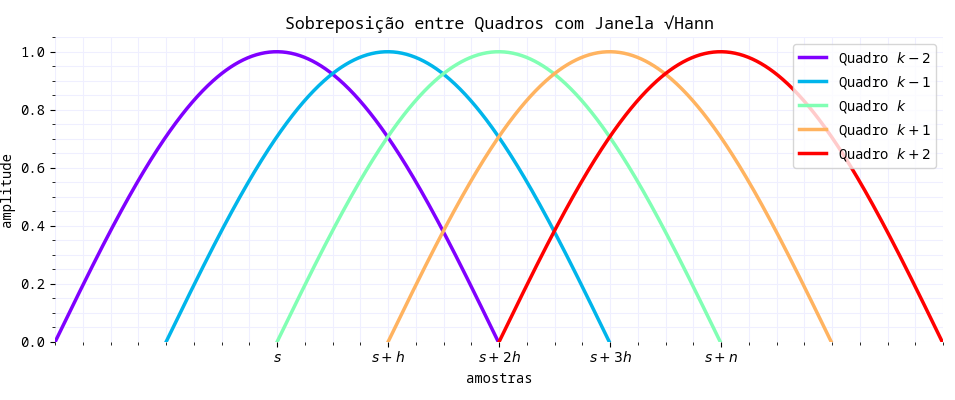
\includegraphics[width=\linewidth]{figures/overlap-add.png}
    \caption{Sobreposição entre quadros utilizando janela raiz de Hann e taxa de sobreposição de 75\%.}
    \label{fig:overlap-add}
\end{figure}

Como múltiplos quadros sobrepostos contribuem simultaneamente para uma mesma região temporal do sinal reconstruído, torna-se necessário aplicar um fator de normalização durante a síntese. Esse procedimento evita variações artificiais de amplitude causadas pela superposição das janelas.

\subsection{Estimação de Frequência pelo \textit{Phase Vocoder}}

Após a obtenção do espectro complexo de cada quadro, o algoritmo extrai a magnitude e a fase associadas a cada \textit{bin} espectral. As fases do quadro anterior são armazenadas para permitir a análise da evolução temporal de cada componente entre quadros consecutivos.

O avanço de fase esperado para cada \textit{bin} é calculado em função de sua frequência central, do tamanho da FFT e do intervalo entre análises. Em seguida, o algoritmo calcula a diferença entre as fases observadas em quadros consecutivos.

\begin{minted}{cpp}
float deltaPhase = phase - previousAnalysisPhases[k];

float expectedPhaseAdvance =
    tau * static_cast<float>(k)
    * static_cast<float>(analysisHopSamples)
    / static_cast<float>(frameSamples);
\end{minted}

Como fases são representadas modularmente no intervalo \([-\pi, \pi]\), diferenças de fase podem apresentar ambiguidades causadas por rotações completas do círculo trigonométrico. Para corrigir esse efeito, a diferença entre o avanço observado e o avanço esperado é normalizada para o intervalo angular principal.

\begin{minted}{cpp}
float residualPhase = wrapAngle(
        deltaPhase - expectedPhaseAdvance
    );
\end{minted}

A partir desse resíduo de fase, o algoritmo estima a frequência angular efetiva de cada componente espectral.

\begin{minted}{cpp}
float trueFrequency =
    tau * static_cast<float>(k)
    / static_cast<float>(frameSamples);

trueFrequency +=
    residualPhase
    / static_cast<float>(analysisHopSamples);
\end{minted}

As frequências estimadas são posteriormente utilizadas durante o processo de deslocamento espectral e síntese do sinal reconstruído.

\subsection{Pitch Shifting no Domínio da Frequência}

Após a estimação das frequências instantâneas, o algoritmo realiza o deslocamento das frequências do sinal segundo a razão correspondente ao número de semitons desejado.

\begin{minted}{cpp}
float pitchRatio = std::pow(2.0f, semitones / 12.0f);
\end{minted}

Para cada \textit{bin} da FFT, a nova posição e a nova frequência estimada são obtidas multiplicando-se os valores originais pela razão calculada.

\begin{minted}{cpp}
shiftedBins[k] = static_cast<float>(k) * pitchRatio;

shiftedFrequency[k] = trueFrequency * pitchRatio;
\end{minted}

Como as novas posições raramente coincidem exatamente com os \textit{bins} discretos da FFT, o algoritmo utiliza interpolação para estimar os valores intermediários necessários para a reconstrução do novo espectro. Esse procedimento permite deslocar as frequências do sinal preservando sua distribuição geral antes da etapa de síntese.

\subsection{Síntese e Reconstrução Temporal}

Após o deslocamento das frequências do sinal, o algoritmo reconstrói um novo espectro complexo utilizando as magnitudes interpoladas e as fases acumuladas durante a síntese.

As fases de síntese são atualizadas continuamente a partir das frequências instantâneas estimadas para cada \textit{bin}, garantindo coerência temporal entre quadros consecutivos.

\begin{minted}{cpp}
synthesisPhases[k] += interpolatedFrequency[k] * static_cast<float>(synthesisHopSamples);
synthesisPhases[k] = wrapAngle(synthesisPhases[k]);
\end{minted}

Em seguida, os coeficientes complexos do novo espectro são reconstruídos a partir das magnitudes e fases sintetizadas.

\begin{minted}{cpp}
buffer[k] = std::polar(interpolatedMagnitude[k], synthesisPhases[k]);
\end{minted}

Após a reconstrução do espectro completo, o algoritmo aplica a transformada inversa para retornar ao domínio do tempo.

Os quadros reconstruídos são então acumulados no buffer de síntese por meio da técnica de \textit{overlap-add}. Durante esse processo, o sinal é novamente multiplicado pela função de janela e normalizado para compensar a superposição entre quadros consecutivos.

\begin{minted}{cpp}
synthesisBuffer[index] +=
    buffer[i].real()
    * window[i]
    / normalization[i];
\end{minted}

\subsection{Considerações Práticas}

A implementação desenvolvida neste trabalho utiliza uma abordagem relativamente direta de \textit{phase vocoder}, baseada na estimação independente das frequências associadas a cada \textit{bin} da FFT. Embora essa estratégia seja suficiente para realizar \textit{pitch shifting} em tempo real, ela pode produzir inconsistências perceptíveis em sinais complexos, especialmente em regiões transientes ou com grande densidade harmônica.

Na literatura, diferentes técnicas são utilizadas para reduzir esses efeitos. Métodos de \textit{phase locking} \cite{laroche1999}, por exemplo, buscam preservar relações de fase entre componentes vizinhas do espectro, reduzindo características artificiais frequentemente associadas ao \textit{phase vocoder}. Outras abordagens utilizam rastreamento de picos espectrais (\textit{peak tracking}) \cite{laroche1999} para acompanhar componentes harmônicas de forma mais estável ao longo do tempo.

Além disso, a escolha do tamanho da FFT influencia diretamente o comportamento do algoritmo. Quadros maiores aumentam a resolução em frequência e melhoram a estimação das componentes do sinal, mas também introduzem maior latência e custo computacional. Quadros menores reduzem a latência ao custo de menor precisão na representação das frequências analisadas.

Durante o deslocamento das frequências, componentes próximas à frequência de Nyquist podem ultrapassar o limite representável pela transformada, deixando de ser reconstruídas corretamente. Da mesma forma, deslocamentos negativos tendem a concentrar múltiplas frequências em regiões mais estreitas do espectro, aumentando a dependência da etapa de interpolação.